% PM template 2014
\documentclass[11pt,a4paper]{book} % this document uses 'book' template
\usepackage[utf8]{inputenc} % set input encoding (not needed with XeLaTeX)
\usepackage[czech]{babel} % we're Czech
\usepackage{amsfonts,multirow,float,enumerate, amsmath,amssymb,amsthm,algorithm,algorithmicx,algpseudocode}

% just some misc pdf magic
\usepackage{ifpdf}
\ifpdf
    \usepackage[pdftex]{graphicx}   % to include graphics
    \pdfcompresslevel=9 
    \usepackage[pdftex,     % sets up hyperref to use pdftex driver
            plainpages=false,   % allows page i and 1 to exist in the same document
            breaklinks=true,    % link texts can be broken at the end of line
            colorlinks=true,
            pdfauthor=Petr Mánek
           ]{hyperref} 
    \usepackage{thumbpdf}
\else 
    \usepackage{graphicx}       % to include graphics
    \usepackage{hyperref}       % to simplify the use of \href
\fi 

\usepackage{pgfplots,dot2texi,tikz} % we like charts
\usetikzlibrary{shapes,arrows,hobby,backgrounds,calc,trees}
\usepackage{caption,subfigure}

\usepackage[margin=3cm]{geometry} % change page margins to 3cm

% theorems and proofs
\newenvironment{t_proof}[1][\proofname]{%
  \begin{proof}[#1]$ $\par\nobreak\ignorespaces
}{%
  \end{proof}
}

\newtheorem{t_theorem}{Věta}[section]

\newtheorem{t_lemma}[t_theorem]{Lemma}
\newtheorem{t_claim}[t_theorem]{Tvrzení}
\newtheorem{t_fact}[t_theorem]{Fakt}

\newtheorem{t_corollary}{Důsledek}[t_theorem]
\newtheorem{t_remark}{Poznámka}[t_theorem]

\theoremstyle{definition}
\newtheorem{t_definition}[t_theorem]{Definice}
\newtheorem*{t_observation}{Pozorování}
\newtheorem*{t_example}{Příklad}
\newtheorem*{t_exercise2}{Příklady k procvičení}
\newenvironment{t_exercise}{%
  \begin{t_exercise2}$ $\par\nobreak\ignorespaces
  \begin{enumerate}
}{%
  \end{enumerate}
  \end{t_exercise2}
}

% document title stuff
\usepackage{titling}
\title{Informatické poznámky}
\author{Petr Mánek}
\date{\today}

% algorithmic macro
\algnewcommand\algorithmicto{\textbf{to}}
\renewcommand{\algorithmicrequire}{\textbf{Vstup:}}
\renewcommand{\algorithmicensure}{\textbf{Výstup:}}
\algrenewtext{For}[3]%
  {\algorithmicfor\ $#1 \gets #2$ \algorithmicto\ $#3$ \algorithmicdo}

% translation and numbering
\makeatletter
\renewcommand{\ALG@name}{Algoritmus}
\@addtoreset{algorithm}{section}
\makeatother
\renewcommand{\thealgorithm}{\thesection.\arabic{algorithm}}
\renewcommand{\restriction}{\mathord{\upharpoonright}}

% header and footer
\usepackage{fancyhdr}
\renewcommand{\subsectionmark}[1]{%
  \ifsubsectioninheader
    \def\subsectiontitle{: #1}%
  \else
    \def\subsectiontitle{}%
  \fi}
\newif\ifsubsectioninheader
\def\subsectiontitle{}
\fancyhf{}
\fancyhead[LE,RO]{\bfseries\thepage}
\fancyhead[LE]{\small \theauthor}
\fancyhead[RO]{\small \nouppercase{\rightmark\ifsubsectioninheader\subsectiontitle\fi}}
\fancyfoot[LE,RO]{\thepage}
\renewcommand{\headrulewidth}{0.5pt}
\renewcommand{\footrulewidth}{0pt}
\fancyheadoffset[RE,LO]{-0.5\textwidth}
\pagestyle{fancy}

\begin{document}
% some other title stuff
\frontmatter
\maketitle

%\tableofcontents
%\chapter{Úvod}
%To do...

% the actual content begins here
\mainmatter
\chapter{Kombinatorika}
% intro ke kombinatorice
\section{Kombinatorické odhady}
V této části se budeme zabývat odhady veličin často používaných při řešení kombinatorických problémů. Na začátek ale zadefinujeme dva klíčové pojmy, bez kterých se neobejdeme.

\begin{t_definition}
  Pro $n\in\mathbb{N}$ definujeme faktoriál jako $n!=1\cdot 2\cdot 3\dots n$. Speciálně, nechť je $0!$ roven 1.
\end{t_definition}

\begin{t_definition}
  Pro $n,k\in\mathbb{N}, k\leq n$ definujeme kombinační číslo $\binom{n}{k}=\frac{n!}{k!(n-k)!}$. Kombinačnímu číslu $\binom{n}{k}$ také říkáme binomický koeficient, ve výrazech jej čteme \textit{$n$ nad $k$}.
\end{t_definition}

\begin{t_observation}
  Platí následující identity: $\binom{n}{k}=\binom{n}{n-k}$, $\binom{n}{0}=\binom{n}{n}=1$, $\binom{n}{1}=\binom{n}{n-1}=n$
\end{t_observation}

\begin{t_theorem}[odhad faktoriálu]
  Nechť $n\in\mathbb{N}$, potom platí:
  \begin{align*}
    e\left(\frac{n}{e}\right)^n\leq n! \leq en\left(\frac{n}{e}\right)^n
  \end{align*}
\end{t_theorem}

\begin{t_proof}[Důkaz (indukcí přes $n$)]
  Pro $n=1$ je rovnost zredukována na $1\leq 1\leq 1$. Můžeme tedy přikročit k indukčnímu kroku. V něm dokážeme každou nerovnost zvlášť. Nejprve se podíváme na horní mez. Z indukčního předpokladu vyplývá následující nerovnost.
  \begin{align*}
    n! = n(n-1)! &\leq en(n-1)\left(\frac{n-1}{e}\right)^{n-1}
  \end{align*}
  Tuto nerovnost můžeme dále ekvivalentně upravovat.
  \begin{align*}
    en(n-1)\left(\frac{n-1}{e}\right)^{n-1}
    &= en\frac{(n-1)^n}{e^{n-1}}\\
    &= en\frac{(n-1)^n}{e^{n-1}}\cdot\frac{n^n}{n^n}\cdot\frac{e}{e}\\
    &= en\left(\frac{n}{e}\right)^n\cdot e\left(\frac{n-1}{n}\right)^n\\
    &= en\left(\frac{n}{e}\right)^n\cdot e\left(1-\frac{1}{n}\right)^n
  \end{align*}
  Nyní použijeme fakt, že $\left(1-\frac{1}{n}\right)^n\leq \frac{1}{e}$, a nerovnost doupravíme do požadované formy.
  \begin{align*}
    en\left(\frac{n}{e}\right)^n\cdot e\left(1-\frac{1}{n}\right)^n
    &\leq en\left(\frac{n}{e}\right)^n\cdot \left(\frac{1}{e^n}\right)^n\\
    &= en\left(\frac{n}{e}\right)^n
  \end{align*}
  Tím je důkaz pravé nerovnosti hotov. Nyní provedeme analogickou úvahu i pro levou nerovnost, začneme opět u indukčního předpokladu.
  \begin{align*}
    n! = n(n-1)! &\geq en\left(\frac{n-1}{e}\right)^{n-1}
  \end{align*}
  Provedeme podobné ekvivalentní úpravy jako u minulého případu.
  \begin{align*}
    en\left(\frac{n-1}{e}\right)^{n-1}
    &= en\left(\frac{n-1}{e}\right)^{n-1}\cdot\frac{n^n}{n^n}\cdot\frac{e}{e}\\
    &= e\left(\frac{n-1}{n}\right)^{n-1}\cdot\frac{n^ne}{e^{n}}\\
    &= \frac{e^2\left(\frac{n}{e}\right)^n}{\left(\frac{n}{n-1}\right)^{n-1}}\\
    &= \frac{e^2\left(\frac{n}{e}\right)^n}{\left(1+\frac{1}{n-1}\right)^{n-1}}
  \end{align*}
  Přišel čas na připomenutí faktu, že $\left(1-\frac{1}{n}\right)^n\leq \frac{1}{e}$. Jelikož je však část výrazu ve jmenovateli, nesmíme zapomenout nerovnost otočit.
  \begin{align*}
    \frac{e^2\left(\frac{n}{e}\right)^n}{\left(1+\frac{1}{n-1}\right)^{n-1}}
    &\geq \frac{e^2\left(\frac{n}{e}\right)^n}{\left(e^{\frac{1}{n-1}}\right)^{n-1}}\\
    &= \frac{e^2\left(\frac{n}{e}\right)^n}{e}\\
    &= e\left(\frac{n}{e}\right)^n
  \end{align*}
  Podařilo se nám tedy úspěšně dokázat horní i dolní mez pro faktoriál. Důkaz je dokončen.
\end{t_proof}

Ukazuje se, že tento odhad bohužel není příliš těsný. Lepší aproximaci poskytuje takzvaná Stirlingova formule. Její důkaz ale vyžaduje netriviální využití gamma funkce, proto jej zde vynecháme.
\begin{t_fact}[Stirlingova formule]
  Nechť $n\in\mathbb{N}$, potom platí:
  \begin{align*}
    n! \approx \sqrt{2\pi n}\left(\frac{n}{e}\right)^n
  \end{align*}  
\end{t_fact}

Stirlingův odhad faktoriálu je ve skutečnosti natolik těsný, že jej můžeme využít k velmi dobrému odhadu kombinačních čísel. Stačí jej substituovat do vzorce $\frac{n!}{k!(n-k)!}$. Jediná slabina tohoto odhadu je, že je jako matematický výraz příliš komplikovaný. Proto si ukážeme odhad, který je o epsilon horší, ale zároveň výrazně jednodušší.

\begin{t_theorem}[odhad kombinačního čísla]
  Nechť $n,k\in\mathbb{N}$, $k\leq n$, potom platí:
  \begin{align*}
    \left(\frac{n}{k}\right)^k\leq \binom{n}{k}\leq \frac{1}{e}\cdot\left(\frac{en}{k}\right)^k
  \end{align*}
\end{t_theorem}
\begin{t_proof}
  \begin{align*}
    \binom{n}{k}=\frac{n(n-1)\dots(n-k+1)}{k!}
    \leq \frac{n^k}{k!}
    \leq \frac{n^k}{e\left(\frac{k}{e}\right)^k}
    = \frac{1}{e}\cdot\left(\frac{en}{k}\right)^k
  \end{align*}
  
  Důkaz dolního odhadu bude trochu komplikovanější, budeme k němu muset použít oba odhady faktoriálu, které jsme dokázali dříve. Protože odhadujeme celý zlomek, musíme ve jmenovateli opět použít opačný odhad.
  \begin{align*}
    \binom{n}{k}
    = \frac{n!}{k!(n-k)!}
    \geq \frac{en\left(\frac{n}{e}\right)^n}{e\left(\frac{k}{e}\right)^ke\left(\frac{n-k}{e}\right)^{n-k}}
    = \frac{n^{n+1}}{k^k(n-k)^{n-k}}
  \end{align*}
  
  Hodně mocnin se nám podařilo zkrátit, nyní musíme postupovat ekvivalentními úpravami.
  \begin{align*}
    \frac{n^{n+1}}{k^k(n-k)^{n-k}}
    &\stackrel{?}{\geq} \left(\frac{n}{k}\right)^k=\frac{n^k}{k^k}\\
    \frac{n^{n+1}}{(n-k)^{n-k}}
    &\stackrel{?}{\geq} n^k\\
    n\cdot \frac{n^{n-k}}{(n-k)^{n-k}}
    &\stackrel{?}{\geq} 1\\
    n\cdot\underbrace{\left(\frac{n}{n-k}\right)^{n-k}}_{\geq 1}
    &\geq 1
  \end{align*}
\end{t_proof}

Z uvedeného odhadu vyplývá speciální případ pro centrální binomické koeficienty.
\begin{t_corollary}
  Nechť $n\in\mathbb{N}$, potom platí:
  \begin{align*}
    2^n\leq \binom{2n}{n}\leq 2^ne^{n-1}
  \end{align*}
\end{t_corollary}

\begin{t_exercise}
  \item Porovnejte $\binom{80}{20}$, $\binom{90}{20}$, $\binom{90}{80}$, $\binom{80}{60}$, $\binom{90}{30}$, $\binom{80}{10}$.
  \item Porovnejte $n!$, $\binom{2n}{n}$, $\binom{2n}{n-1}$, $n^{\sqrt{n}}$, $\sqrt{n}^n$.
  \item Spočítejte, kolik nulových cifer je na konci dekadického zápisu čísla $12723!$.
  \item Rozhodněte, která z následujících funkcí roste asymptoticky rychleji:
  \\$f(n)=\binom{10n}{\lceil\sqrt{n}\rceil}$ nebo $g(n)=n^\sqrt{n}$.
  \item Rozhodněte, která z následujících funkcí roste asymptoticky rychleji. Funkce $f(n)$ označuje počet podmnožin velikosti $n$ množiny obsahující $2n$ prvků. Funkce $g(n)$ označuje počet podmnožin velikosti nejvýše $0,999n$ množiny obsahující $2n$ prvků.
  \item Označme $r(n)$ počet rovinných grafů na množině vrcholů $1\dots n$ a $g(n)$ na stejné množině vrcholů. Dokažte, že pro každé dostatečně velké $n$ platí:
  \begin{align*}
    r(\lfloor n^{1,999} \rfloor)<g(n)<r(n^2)
  \end{align*}
  \item Kolik z přirozených čísel $1\dots 420$ není dělitelných 6, 17 ani 42?
  \item Kolik různých (ne nutně smysluplných) slov vznikne permutací písmen slova \textit{abrakadabra}? Slovem myslíme jen posloupnost znaků.
\end{t_exercise}     % petrmanek
\section{Vytvořující funkce}
\begin{t_definition}
  Vytvořující funkce posloupnosti $\{a_n\}_{n=0}^\infty$ je funkce $A:\mathbb{R}\rightarrow\mathbb{R}$ definovaná $A(x)=a_0+a_1x+a_2x^2+a_3x^3+\dots=\sum_{i\geq 0}a_ix^i$.
\end{t_definition}

\begin{t_example}
  Jak spočítáme všechna binární slova, tedy řetězce složené pouze z jedniček a nul? Řetězců délky $k$ je $2^k$, protože každé z $k$ míst můžeme zaplnit právě jednou ze 2 možností, jedničkou nebo nulou. Pokud počet řetězců délky $k$ označíme jako  $a_k=2^k$, získáme rostoucí geometrickou posloupnost $1,2,4,8,16,\dots$.
  
  Vytvořující funkce této posloupnosti bude $A(x)=1+2x+4x^2+8x^3+16x^4+\dots$. Pro $|x|<1$ tato řada konverguje k hodnotě $\frac{1}{1-2x}$. Tento předpoklad pro argument vytvořující funkce budeme používat i nadále. Můžeme tedy psát $A(x)=\frac{1}{1-2x}$.
\end{t_example}

\begin{t_observation}
  Posloupnost $a_n=1$ má vytvořující funkci $A(x)=\frac{1}{1-x}$. Obecněji, posloupnost $b_n=q^n$ ($q\in\mathbb{R}$) má vytvořující funkci $B(x)=\frac{1}{1-qx}$.
\end{t_observation}

\begin{t_fact}
  Pro každou posloupnost existuje vytvořující funkce. Posloupnost je touto vytvořující funkcí jednoznačně určena (až na ekvivalentní úpravy).
\end{t_fact}

\begin{t_example}[řešení lineární rekurence]$ $\\
  Mějme posloupnost $\{a_n\}_{n=0}^\infty$ zadanou rekurentně, naším úkolem je najít explicitní vzorec.
  \begin{align*}
    a_n =
    \begin{cases}
      2 & n = 0 \\
      5 & n = 1 \\
      5a_{n+1}-6a_n & n\geq 2
    \end{cases}
  \end{align*}
  
  Předpokládejme, že $a_n$ má vytvořující funkci $A(x)=a_0+a_1x+a_2x^2+a_3x^3+\dots$. Podle výše zadaného rekurentního vztahu musí platit následující rovnice.
  \begin{align*}
    0=a_{n+2}-5a_{n+1}+6a_n
  \end{align*}
  
  Pokusíme se tohoto vztahu využít pro získání tvaru vytvořující funkce $A(x)$. Podle ní potom určíme explicitní vzorec pro $n$-tý člen. Pojďme nyní funkci $A(x)$ vynásobit a sečíst.
  \begin{align*}
    A(x) &= a_0+a_1x+a_2x^2+a_3x^3+\dots\\
    -5xA(x) &= -5a_0x-5a_1x^2-5a_2x^3-5a_3x^4+\dots\\
    6x^2A(x) &= 6a_0x^2+6a_1x^3+6a_2x^4+6a_3x^5+\dots\\
    (1-5x+6x^2)A(x) &= a_0+(a_1-5a_0)x+\underbrace{(a_2-5a_1+6a_0)}_{=0}x^2+\underbrace{(a_3-5a_2+6a_1)}_{=0}x^3+\dots
  \end{align*}
  
  Díky tomu, jak se nám podařilo funkci povytýkat a sečíst, můžeme aplikovat rekurentní rovnici, která od kvadratického členu dále vynuluje koeficienty. Tímto způsobem se vcelku elegantně zbavíme nekonečně mnoha neznámých a zbyde nám vzorec omezený na počáteční body rekurence, ze kterého vytvořující funkci snadno vyjádříme.
  \begin{align*}
    (1-5x+6x^2)A(x) &= a_0+(a_1-5a_0)x\\
    (1-5x+6x^2)A(x) &= 2-5x\\
    A(x) &= \frac{2-5x}{1-5x+6x^2}
  \end{align*}
  
  Máme tedy vytvořující funkci. Co nám to ale říká o posloupnosti? Jak uvidíme dále, z vytvořující funkce můžeme bez větší námahy získat explicitní vzorec pro posloupnost, za předpokladu, že známe vytvořující funkce nejčastějších posloupností a umíme na ně složitější výrazy rozložit. V tomto konkrétním případě použijeme úpravu na parciální zlomky.
  \begin{align*}
    A(x) &= \frac{2-5x}{1-5x+6x^2}\\
    A(x) &= \frac{2-5x}{(1-2x)(1-3x)}\\
    A(x) &= \underbrace{\frac{1}{1-2x}}_{2^n}+\underbrace{\frac{1}{1-3x}}_{3^n}
  \end{align*}
  
  V tomto tvaru vypadá vytvořující funkce mnohem jednodušeji a je také lépe identifikovatelná. Pokud využijeme pozorování o geometrických posloupnostech a jejich vytvořujících funkcích, zjistíme, že levý zlomek je vytvořující funkcí posloupnosti $2^n$ a pravý zlomek je vytvořující funkcí posloupnosti $3^n$. Díky linearitě vytvořujících funkcí, kterou brzy podrobněji rozebereme, můžeme tedy náš výpočet uzavřít a určit explicitní vzorec pro posloupnost $a_n$.
  \begin{align*}
    A(x) &= \sum_{i\geq 0}(2^i+3^i)x^i\\
    a_n&=2^n+3^n
  \end{align*}
\end{t_example}

\begin{t_fact}[časté vytvořující funkce]
  Nechť $\{a_n\}_{n=0}^\infty$, $\{b_n\}_{n=0}^\infty$ jsou posloupnosti, $A(x)$, $B(x)$ jejich odpovídající vytvořující funkce a $\alpha\in\mathbb{R}$, potom platí:
  \begin{enumerate}
    \item $A(x)+B(x)$ je vytvořující funkce posloupnosti $a_n+b_n$.
    \item $A(\alpha x)$ je vytvořující funkce posloupnosti $\alpha^n\cdot a_n$.
    \item $\alpha A(x)$ je vytvořující funkce posloupnosti $\alpha\cdot a_n$.
    \item $x\cdot A^\prime(x)$ je vytvořující funkce posloupnosti $n\cdot a_n$.
  \end{enumerate}   
 \end{t_fact}
 
\begin{t_fact}[vytvořující funkce a posun posloupnosti]
  Nechť $\{a_n\}_{n=0}^\infty$ je posloupnost, $A(x)$ její vytvořující funkce a $k \in\mathbb{N}$, potom platí:
  \begin{enumerate}
    \item $x^k\cdot A(x)$ je vytvořující funkce posloupnosti $\underbrace{0, 0, 0, 0, 0, 0}_{k}, a_0, a_1, a_2\dots$.
    \item $A(x^k)$ je vytvořující funkce posloupnosti $a_0, \underbrace{0, 0, 0, 0}_{k}, a_1, \underbrace{0, 0, 0, 0}_{k}, a_2,\dots$.
  \end{enumerate}
\end{t_fact}

\begin{t_definition}[zobecněné kombinační číslo]
  Pro $r\in\mathbb{R}$, $k\in\mathbb{Z}$ a $k\geq 0$ definujeme zobecněné kombinační číslo $\binom{r}{k}=\frac{r(r-1)(r-2)\dots (r-k+1)}{k!}$.
\end{t_definition}

\begin{t_lemma}
  Nechť $n,k\in\mathbb{N}$, potom platí:
  \begin{align*}
    \binom{-n}{k}=(-1)^k\binom{n+k-1}{n-1}
  \end{align*}
\end{t_lemma}

\begin{t_proof}[Důkaz (přímočarý)]
  \begin{align*}
    \binom{-n}{k}&=\frac{(-n)(-n-1)\dots(-n-k+1)}{k!}=
    (-1)^k\frac{n(n+1)\dots(n+k-1)}{k!}=\\
    &=(-1)^k\frac{(n+k-1)!}{k!(n-1)!}=(-1)^k\binom{n+k-1}{n-1}
  \end{align*}
\end{t_proof}

\begin{t_fact}[zobecněná binomická věta]
  Nechť $r\in\mathbb{R}$, potom $\forall x :|x|<1$ platí:
  \begin{align*}
    (1+x)^r=\sum_{k\geq 0}\binom{r}{k}x^k
  \end{align*}
\end{t_fact}

\begin{t_example}
  Zjistíme vytvořující funkci posloupnosti $a_n=\frac{1}{(1-n)^3}$.
  \begin{align*}
    \frac{1}{(1-x)^3}=(1-x)^{-3}
    =\sum_{k\geq 0}\binom{-3}{k}(-x)^k
    =\sum_{k\geq 0}\binom{-3}{k}x^k(-1)^k
  \end{align*}
  
  Nejprve si posloupnost zapíšeme jako jmenovatel se záporným exponentem, poté využijeme zobecněnou binomickou větu, abychom výraz převedli na mocninnou řadu.
  \begin{align*}
    \sum_{k\geq 0}\binom{-3}{k}x^k(-1)^k
    =\sum_{k\geq 0}(-1)^k\binom{3+k-1}{2}x^k(-1)^k
    =\sum_{k\geq 0}\binom{k+2}{2}x^k
  \end{align*}
  
  Aplikujeme lemma, která nám umožní převést kombinační číslo do jednoduššího tvaru. Vytvořující funkce $A(x)$ posloupnosti $a_n$ je tedy definována následujícím výrazem. 
  \begin{align*}
    A(x)=\binom{k+2}{2}
  \end{align*}
\end{t_example}

\begin{t_exercise}
  \item Sečtěte řady $\sum_{k=0}^n \binom{n}{k}^2$, $\sum_{k=0}^n (-1)^k\binom{n}{k}^2$, $\sum_{k=0}^n k\binom{n}{k}$, $\sum_{k=0}^n k^2\binom{n}{k}^2$.
  \item Určete hodnotu koeficientu u $x^{13}$ v $(x^2+x^3+x^4+\dots)^4$.
  \item Určete hodnotu koeficientu u $x^4$ v $\sqrt[3]{1+x}$.
  \item Určete hodnotu koeficientu u $x^5$ v $\frac{1}{(1-2x)^2}$.
  \item Najděte vytvořující funkce pro posloupnosti $(1, 1, 1, 1, \dots)$, $(1, 2, 3, 4, \dots)$, $(2, 4, 6, 8, \dots)$.
  \item Najděte vytvořující funkce pro posloupnosti $(1, 3, 5, 7, \dots)$, $(1, 0, 1, 0, \dots)$, $(1, -3, 5, -7, \dots)$.
  \item Najděte explicitní vzorec pro posloupnost zadanou rekurentně: $a_0=2, a_1=3$ a $a_{n+2}+2a_{n+1}-3a_n=0$ pro $n\geq 2$.
  \item Najděte explicitní vzorec pro posloupnost zadanou rekurentně: $a_0=1, a_1=1$ a $a_{n+2}-a_{n+1}-6a_n=0$ pro $n\geq 2$.
  \item Najděte explicitní vzorec pro posloupnost zadanou rekurentně: $a_0=0, a_1=1$ a $a_{n+2}=4(a_{n+1}-a_n)$ pro $n\geq 2$.
  \item Spočítejte všechny řetězce o délce $n$ sestavené pouze z nul a jedniček takové, že se žádné dva po sobě jdoucí znaky nejsou nuly. Odpověď vyjádřete formou rekurentní posloupnosti.
  \item Najděte explicitní vzorec pro posloupnost z předchozí úlohy.
\end{t_exercise}   % petrmanek
\section{Konečné projektivní roviny}
\begin{t_definition}
  Konečná projektivní rovina je dvojice $(X, \mathcal{L})$, kde $X$ je konečná množina bodů a $\mathcal{L}\subseteq 2^X$ je množina přímek taková, že následující axiomy jsou splněny:
  \begin{enumerate}
    \item[(A1)]
    \textit{Každé dvě různé přímky se protínají v právě jednom bodě.}
    \\$\forall K,L\in\mathcal{L},K\neq L : |K\cap L|=1$
    \item[(A2)]
    \textit{Každé dva různé body určují právě jednu přímku.}
    \\$\forall x,y\in X,x\neq y : \exists! L\in\mathcal{L} : \{x, y\}\subseteq L$
    \item[(A0)]
    \textit{Existuje čtveřice bodů taková, že žádné tři body z ní neleží na společné přímce.}
    \\$\exists Č\in\binom{X}{4}:\forall L\in\mathcal{L}:|Č\cap L|\leq 2$
  \end{enumerate}
\end{t_definition}

\begin{t_example}[Fanova rovina]$ $
  \begin{figure}[!htbp]
    \centering
    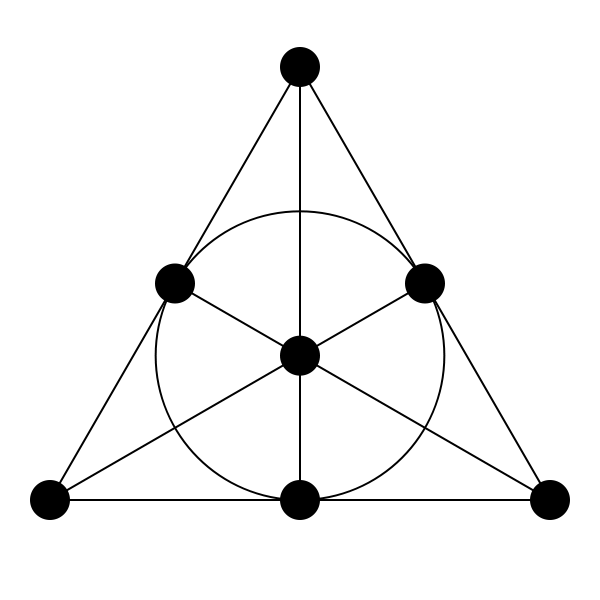
\includegraphics[width=0.5\textwidth]{img/fano_plane.png}
  \end{figure}
\end{t_example}

\begin{t_lemma}[o dvou přímkách]
  Nechť $(X, \mathcal{L})$ je konečná projektivní rovina, potom platí, že pro každou dvojici přímek existuje bod, který na nich neleží:
  \begin{align*}
    \forall K, L\in\mathcal{L} : \exists x\in X : x\notin K\cup L
  \end{align*}
\end{t_lemma}
\begin{t_proof}
  Uvažme množinu $Č$ z axiomu (A0) a libovolné dvě různé přímky $K, L\in\mathcal{L}$. Podle axiomu (A0) musí platit, že $K$ i $L$ každá protíná nejvýše 2 body z $Č$. Ekvivalentně zapsáno $|K\cap Č|\leq 2$ a $|L\cap Č|\leq 2$. To znamená, že $|(K\cup L)\cap Č|\leq 4$.
  
  Rozlišíme dva případy:
  \begin{enumerate}
    \item Pokud $|(K\cup L)\cap Č|\leq 3$, musí existovat alespoň jeden bod z $Č$, který nenáleží $K$ ani $L$. Vybereme tedy libovolný bod $x\in Č\setminus(K\cup L)$.
    \item Pokud $|(K\cup L)\cap Č|= 4$, je zřejmé, že $K$ a $L$ má v $Č$ právě dva průsečíky, označme je $K\cap Č=\{a,b\}$ a $L\cap Č=\{c,d\}$.
    
    Zaveďme označení $\overline{xy}$ pro přímku určenou body $x$ a $y$. Doplníme, že podle (A2) musí vždy taková přímka existovat a musí být určena jednoznačně až na pořadí bodů. Jednoduché pozorování je, že $\overline{ab}$ je $K$ a $\overline{cd}$ je $L$.
    
    Podle (A1) musí mít přímky $\overline{ac}$ a $\overline{bd}$ průsečík $x=\overline{ac}\cap\overline{bd}$. Víme ale také, že bod $x$ nemůže ležet na $K$, protože by přímka $K$ měla spolu s přímkami $\overline{ac}$, $\overline{bd}$ dvojice průsečíků $\{a,x\}$ a $\{b,x\}$, což by porušilo axiom (A1). Analogicky bod $x$ nemůže ležet ani na $L$.
    
    Bod $x$ tedy má vlastnost, kterou jsme hledali, a důkaz je dokončen.
  \end{enumerate}
\end{t_proof}

\begin{t_theorem}[o řádu roviny]
  Nechť $(X, \mathcal{L})$ je konečná projektivní rovina, potom platí, že každá přímka protíná stejný počet bodů. Ekvivalentně:
  \begin{align*}
    \forall K, L\in\mathcal{L}:|K|=|L|
  \end{align*}
\end{t_theorem}

\begin{t_proof}
  Uvažme libovolné dvě přímky $K, L\in\mathcal{L}$. Podle předchozího lemmatu musí existovat bod $x\in X$, který na nich neleží. Můžeme zavést zobrazení $f:K\rightarrow L$ definované tak, že obrazem bodu $t$ je průsečík přímky $\overline{xt}$ a $L$, formálněji: $f(t)=\overline{xt}\cap L$. 
  
  Nyní ukážeme, že $f$ je bijekce, z čehož vyplývá, že přímky $K$ a $L$ mají stejný počet bodů. Aby zobrazení $f$ bylo vzájemně jednoznačné, musí být zároveň prosté a na. 
  \begin{itemize}
    \item
    Zobrazení $f$ je prosté, protože pokud by existovaly dva body $t_1, t_2\in K$ takové, že $f(t_1)=f(t_2)=s$, znamenalo by to, že přímky $\overline{xt_1}$ a $\overline{xt_2}$ mají dva průsečíky $\{x,s\}$, což je spor s axiomem (A1).
    
    \item
    Zobrazení $f$ je na, protože každý bod $s\in L$ určuje podle axiomu (A2) přímku $\overline{xs}$, která podle axiomu (A1) musí mít průsečík $t\in K$.
  \end{itemize}
\end{t_proof}

\begin{t_definition}
  Řád konečné projektivní roviny $(X,\mathcal{L})$ je $|L|-1$, kde $L\in\mathcal{L}$.
\end{t_definition}

\begin{t_example}
  Fanova rovina je rovinou řádu 2, protože každá přímka protíná právě 3 body.
\end{t_example}

\begin{t_theorem}[vlastnosti řádu]
  Nechť $(X,\mathcal{L})$ je konečná projektivní rovina řádu $n$. Potom platí:
  \begin{enumerate}
    \item
    \textit{Každým bodem prochází $n+1$ přímek.}
    \\$\forall x\in X:|\{L\in\mathcal{L}\mid x\in L\}| = n+1$
    
    \item
    $|X|=n^2+n+1$
    
    \item
    $|\mathcal{L}|=n^2+n+1$
  \end{enumerate}
\end{t_theorem}

\begin{t_proof}
  \begin{enumerate}
    \item
    Uvažme libovolný bod $x\in X$ a přímku $L\in\mathcal{L}$, která jej neobsahuje. Podle předchozí věty musí přímka $L$ obsahovat právě $n+1$ bodů. Tyto body, spolu s bodem $x$, určují podle axiomu (A2) právě $n+1$ různých přímek. Nyní víme, že bodem $x$ prochází alespoň $n+1$ přímek. Nemůžeme si ale být jisti, že jich není více.
    
    Pokud by taková situace nastala, znamenalo by to, že přímka $L$ by s těmito přímkami musela mít společných více než $n+1$ bodů (spor s řádem roviny) nebo by některé z těchto přímek musely protínat stejný bod vícekrát (alespoň dvě přímky mají dva průsečíky). V každém případě bychom došli ke sporu. Bodem $x$ tedy musí procházet právě $n+1$ přímek.
    
    \item
    Uvažme opět stejnou situaci s bodem $x\in X$ a přímkou $L\in\mathcal{L}$, která jej neobsahuje. Na $L$ leží právě $n+1$ bodů, které spolu s bodem $x$ určují $n+1$ různých přímek, označme je $\mathcal{K}=\{K_1, K_2,\dots K_{n+1}\}$.
    
    Na každé přímce $K_i\in\mathcal{K}$ musí ležet také $n+1$ bodů. Víme, že jedním z těchto bodů je bod $x$, který sdílejí všechny přímky z $\mathcal{K}$. Zbylých $n$ bodů na přímce $K_i$ již nemůže ležet na žádné další přímce z $\mathcal{K}$, protože by každý další bod společný dvěma přímkám z $\mathcal{K}$ byl po bodu $x$ jejich druhým průsečíkem, což by porušilo axiom (A1).
    
    V $\mathcal{K}$ tedy musí být vyjma bodu $x$ celkem $(n+1)n=n^2+n$ různých bodů. Přidáme-li k tomuto počtu bod $x$, získáme $n^2+n+1$ bodů, což jsme chtěli dokázat. Úvahu uzavřeme pozorováním, že každý bod z $L$ náleží právě jedné přímce z $\mathcal{K}$ a kromě bodů přímek z $\mathcal{K}$ se v rovině žádný další bod vyskytovat nemůže, jinak by došlo k porušení axiomu (A1). Tím je důkaz hotov.
    
    \item
    Důkaz tohoto bodu je analogický k bodu 2. a vyplývá z duality bodů a přímek v konečných projektivních rovinách.
  \end{enumerate}
\end{t_proof}

\begin{t_definition}
  Množinový systém je dvojice $(X,\mathcal{L})$, kde $X$ je konečná množina a $\mathcal{L}\subseteq 2^X$. Množinu $X$ nazýváme nosnou množinou systému $(X,\mathcal{L})$.
\end{t_definition}

\begin{t_remark}
  Pozorujeme, že každá konečná projektivní rovina je množinovým systémem, ale ne všechny množinové systémy jsou konečnými projektivními rovinami.
\end{t_remark}

\begin{t_example}
  Nechť je $X=\{1,2,3\}$ a $\mathcal{L}=\{\{1,3\},\{1,2\},\{3\}\}$. $(X,\mathcal{L})$ je množinový systém.
\end{t_example}

\begin{t_definition}
  Pro každý množinový systém $(X,\mathcal{L})$ definujeme incidenční graf $(V,E)$, kde $V=X\cup\mathcal{L}$ a $E=\{(x,L)\mid x\in X, L\in\mathcal{L}, x\in L\}$.
\end{t_definition}

\begin{t_remark}
  Incidenční graf množinového systému je bipartitní graf, jehož jedna partita je tvořena prvky nosné množiny a druhá partita množinami v systému. Hrany spojují prvky nosné množiny s množinami v systému, ve kterých jsou tyto prvky obsaženy.
\end{t_remark}

\begin{t_remark}
  Axiomy konečných projektivních rovin je možno interpretovat geometricky na incidenčních grafech. Rozmyslete si, jak by vypadalo jejich znění.
\end{t_remark}

\begin{t_definition}
  Multimnožina je množina, ve které se každý prvek může vyskytnout víckrát než jednou. Můžeme jí jednoduše zkonstruovat pomocí obyčejné množiny a zobrazení, které každému prvku z množiny přiřadí jeho četnost v multimnožině.
\end{t_definition}

\begin{t_example}
  Multimnožinu $\tilde{X}=\{e_1, e_2, e_3, e_2, e_2, e_3\}$ zkonstruujeme použitím obyčejné množiny $X=\{e_1, e_2, e_3\}$ a zobrazení $f:X\rightarrow\mathbb{N}$ takového, že $f(e_1)=1$, $f(e_2)=3$ a $f(e_3)=2$.
\end{t_example}

\begin{t_remark}
  Dále v textu bude každá množina považována za multimnožinu.
\end{t_remark}

\begin{t_definition}
  Pro každý množinový systém $(X,\mathcal{L})$ definujeme jeho duální systém $(Y,\mathcal{M})$ tak, že jejich incidenční grafy jsou isomorfní po výměně partit. Přesněji, $Y=\mathcal{L}$, $\mathcal{M}=\{M_x\mid x\in\mathbb{X}\}$, kde $M_x=\{L\in\mathcal{L}\mid x\in L\}$.
\end{t_definition}

\begin{t_theorem}[o dualitě rovin]
  Duální systém konečné projektivní roviny je konečnou projektivní rovinou stejného řádu.
\end{t_theorem}

\begin{t_proof}
  Mějme konečnou projektivní rovinu $(X,\mathcal{L})$ a její duální systém $(Y,\mathcal{M})$. Aby $(Y,\mathcal{M})$ byl konečnou projektivní rovinou, musí splňovat všechny tři axiomy z definice. Pozorujeme, že axiom (A1) v $(X,\mathcal{L})$ implikuje platnost axiomu (A2) v $(Y,\mathcal{M})$. Stejně tak axiom (A2) v $(X,\mathcal{L})$ implikuje platnost axiomu (A1) v $(Y,\mathcal{M})$. Zbývá ověřit platnost axiomu (A0).
  
  Jestliže v $(X,\mathcal{L})$ existuje čtveřice bodů taková, že žádné tři z nich neleží na jedné přímce, potom musí existovat i čtveřice přímek taková, že žádné tři z nich nemají společný průsečík. Tím je dokázána platnost axiomu (A0) v $(Y,\mathcal{M})$.
\end{t_proof}

\begin{t_corollary}
  Každé tvrzení o konečné projektivní rovině může být díky této dualitě převedeno na jiné ekvivalntní tvrzení.
\end{t_corollary}

\begin{t_theorem}[o existenci rovin]
  Nechť je $n$ mocninou prvočísla, $\mathbb{K}$ těleso s $n$ prvky a $\mathbb{K}^3$ vektorový prostor dimenze 3 nad $\mathbb{K}$, potom existuje konečná projektivní rovina řádu $n$.
\end{t_theorem}

\begin{t_proof}
  Definujeme relaci $\sim$ na $\mathbb{K}$ tak, že $x\sim y\equiv \exists\lambda\in\mathbb{K}, \lambda\neq 0:x=\lambda y$. Nahlédneme, že relace $\sim$ je ekvivalence, pojďme nyní prozkoumat její třídy na $\mathbb{K}^3\setminus 0$. Jejich reprezentanty jsou tyto vektory:
  \begin{itemize}
    \item $(1,\alpha,\beta)$, kde $\alpha,\beta\in\mathbb{K}$ – těchto vektorů je $n^2$,
    \item $(0,1,\alpha)$, kde $\alpha,\in\mathbb{K}$ – těchto vektorů je $n$,
    \item $(0,0,1)$ – pouze jeden vektor.
  \end{itemize}
  
  Vektory budou množinou bodů $X=\mathbb{K}^3\setminus 0$. Pro každý vektor $x\in X$ definujeme přímku $L_x=\{y\in X\mid x\cdot y=0\}$, takto získáme $n^2+n+1$ přímek, které seskupíme v množině $\mathcal{L}=\{L_x\mid x\in X\}$. Aby $(X,\mathcal{L})$ byla konečnou projektivní rovinou, musí splnit axiomy.
  \begin{enumerate}
    \item[(A1)] Máme dvě přímky $L_a, L_b$ a zajímá nás počet bodů, které mají společné. Body $y$ v $L_a$ musí splňovat $a\cdot y=0$, body v $L_b$ musí splňovat $b\cdot y=0$. Společné body obou přímek jsou řešením soustavy těchto dvou rovnic.
    
    Je triviální nahlédnout, že uvedená soustava má vždy právě jedno řešení.
    
    \item[(A2)] Analogickou úvahou.
    
    \item[(A0)] ... % todo
  \end{enumerate}
\end{t_proof}

\begin{t_exercise}
  \item Dokažte, že axiom (A0) můžeme v definici KPR nahradit axiomem (A0a):\\
  \textit{Existují 2 přímky takové, že každá z nich má alespoň 3 body.}
  \\$\exists K, L\in\mathcal{L}:|K|\geq 3\wedge|L|\geq 3$
  
  \item Dokažte, že axiom (A0) můžeme v definici KPR nahradit axiomem (A0b):\\
  \textit{Neexistují 2 přímky takové, že by pokryly všechny body.}
  \\$\forall K, L\in\mathcal{L}:K\cup L\subset X$
  
  \item Pokuste se nakreslit konečnou projektivní rovinu řádu 3.
  
  \item Ukažte, že až na isomorfismus je Fanova rovina jedinou projektivní rovinou řádu 2.
  
  \item Dokažte, že pro nekonečně mnoho různých $n$ existují grafy na $n$ vrcholech s $\Omega(n^\frac{3}{2})$ hranami, které neobsahují jako podgraf $C_4$. Ke konstrukci můžete využít konečné projektivní roviny.
\end{t_exercise}
     % petrmanek
\section{Toky v sítích}
\begin{t_definition}
  Síť je pětice $(V, E, s, t, c)$, kde $G=(V,E)$ je orientovaný graf, $c:E\rightarrow\mathbb{R}$ je zobrazení přiřazující hranám v $G$ jejich kapacitu. Vrcholy $s,t\in V$ jsou zvláštní vrcholy v $G$, které nazýváme jako zdroj a stok.
\end{t_definition}

\begin{t_definition}
  Ohodnocení hran orientovaného grafu $(V,E)$ je funkce $f:E\rightarrow\mathbb{R}$. Pro každé ohodnocení definujeme:
  \begin{enumerate}
    \item \textit{Co do vrcholu přiteče:} $f^+(v)=\sum_{e=(\cdot,v)} f(e)$, kde $v\in V$,
    \item \textit{Co z vrcholu odteče:} $f^-(v)=\sum_{e=(v,\cdot)} f(e)$, kde $v\in V$,
    \item \textit{Přebytek:} $f^\Delta(v)=f^+(v)-f^-(v)$.
  \end{enumerate}
\end{t_definition}

\begin{t_observation}
  Je-li $(V, E, s, t, c)$ síť, potom je funkce $c$ ohodnocením hran grafu $(V,E)$.
\end{t_observation}

\begin{t_definition}
  Tok v síti $(V, E, s, t, c)$ je ohodnocení $f$ takové, že platí:
  \begin{enumerate}
    \item
    \textit{Tok je v mezích kapacity každé hrany.}\\
    $\forall e\in E : 0\leq f(e) \leq c(e)$
    
    \item
    \textit{Kirchhoffův zákon: vstupní tok vrcholu je roven výstupnímu toku.}\\
    $\forall v\in V, v\neq s, t : f^\Delta(v)=0$
  \end{enumerate}
\end{t_definition}

\begin{t_definition}
  Velikost toku $f$ v síti $(V, E, s, t, c)$ definujeme $|f|=-f^\Delta(s)$.
\end{t_definition}

\begin{t_remark}
  Hlavní úlohou teorie toků je hledání tzv. maximálního toku, tedy toku s maximální velikostí. Pojďme si ukázat algoritmus, který tento problém z části řeší.
\end{t_remark}

\begin{t_definition}
  Hladový algoritmus využíváme k nalezení maximálního toku $f$ v síti $(V, E, s, t, c)$. Není ale optimálním algoritmem pro tento druh úlohy!
  
  \begin{algorithm}
    \caption{Hladový algoritmus}
    \begin{algorithmic}[1]
      \State $f\gets$ \textit{nulový tok}
      \Repeat
      \State Najdeme cestu $P$ z vrcholu $s$ do $t$.
      \State Vylepšíme tok $f$ na hranách cesty $P$ na maximální možný.
      \Until{všechny cesty v $G$ jsou nasyceny}
    \end{algorithmic}
  \end{algorithm}
\end{t_definition}

\begin{t_definition}
  Pro srozumitelnost zápisu zavedeme následující označení pro množiny vrcholů $X\subseteq V$ a $Y\subseteq V$ v síti $(V, E, s, t, c)$:
  \begin{enumerate}
    \item $X^+=\{(u,v)\in E\mid u\notin X, v\in X\}$ \textit{množina hran vedoucích do vrcholů v $X$},
    \item $X^-=\{(u,v)\in E\mid u\in X, v\notin X\}$ \textit{množina hran vedoucích z vrcholů v $X$},
    \item $E(X,Y)=\{(u,v)\in E\mid u\in X, v\in Y\}$ \textit{množina hran vedoucích z vrcholů $X$ do $Y$}.
  \end{enumerate}
\end{t_definition}

\begin{t_definition}
  Tokový řez v síti $(V, E, s, t, c)$ je množina $C\subset V$ taková, že $s\in C$, $t\notin C$.
\end{t_definition}

\begin{t_definition}
  Kapacitu řezu $C$ v síti $(V, E, s, t, c)$ definujeme $|C|=\sum_{e\in C^-} c(e)$.
\end{t_definition}

\begin{t_remark}
  Jak uvidíme v dalších větách, maximální tok má úzkou souvislost s tzv. minimálním řezem, tedy řezem, jehož kapacita je minimální.
\end{t_remark}

\begin{t_fact}
  V každé síti existuje maximální tok a minimální řez.
\end{t_fact}

\begin{t_definition}
  Řez $C$ v síti $(V, E, s, t, c)$ je elementární, pokud existuje množina vrcholů $A\subseteq V$ taková, že $s\in A,t\notin A$ a $C=E(A,V\setminus A)$.
\end{t_definition}

\begin{t_lemma}[o elementárním řezu]
  V síti $(V, E, s, t, c)$ každý řez $C$ obsahuje jako podmnožinu elementární řez $A$.
\end{t_lemma}

\begin{t_proof}
  chybí. % todo
\end{t_proof}

\begin{t_corollary}
  Řez je elementární, pokud je minimální v inkluzi.
\end{t_corollary}

\begin{t_definition}
  Pro tok $f$ a řez $C$ v síti $(V, E, s, t, c)$ definujeme:
  \begin{enumerate}
    \item \textit{Co do řezu přiteče:} $f^+(C)=\sum_{e\in C^+} f(e)$,
    \item \textit{Co z řezu odteče:} $f^-(C)=\sum_{e\in C^-} f(e)$,
    \item \textit{Přebytek:} $f^\Delta(C)=f^+(C)-f^-(C)$.
  \end{enumerate}
\end{t_definition}

\begin{t_lemma}[omezení toku řezem]
  Pro každý tok $f$ a řez $C$ v síti $(V, E, s, t, c)$ platí: $|f|=-f^\Delta(C)\leq|C|$.
\end{t_lemma}

\begin{t_proof}
  Nejprve dokážeme rovnost $|f|=-f^\Delta(s)=-f^\Delta(C)$. To uděláme s pomocí matematické indukce. Nahlédneme, že každý řez můžeme sestrojit postupným přidáváním vrcholů do triviálního řezu $\{s\}$. Z definice vyplývá, že $|f|=-f^\Delta(s)=-f^\Delta(\{s\})$. Počáteční podmínka tedy platí. Nyní ukážeme, že při přidání vrcholu do řezu se $f^\Delta$ nezmění.
  
  Mějme řez $C$, pro který platí $-f^\Delta(C)=-f^\Delta(s)$, a vrchol $x\in V, x\neq s, t$ takový, že $x\notin C$. Vytvoříme řez $C^\prime=C\cup x$ a chceme ukázat, že $-f^\Delta(C)=-f^\Delta(C^\prime)$. Uvažme všechny hrany vrcholu $x$, každou hranu $e$ můžeme zařadit do jedné z kategorií:
  \begin{enumerate}
    \item Hrana $e$ vede z $x$ do vrcholu v $C$. Potom její přidání k řezu $C$ sníží $f^-(C)$.
    \item Hrana $e$ vede z vrcholu v $C$ do $x$. Potom její přidání k řezu $C$ sníží $f^+(C)$.
    \item Hrana $e$ vede z $x$ do vrcholu mimo $C$. Potom její přidání k řezu $C$ zvýší $f^+(C)$.
    \item Hrana $e$ vede z vrcholu mimo $C$ do $x$. Potom její přidání k řezu $C$ zvýší $f^-(C)$.
  \end{enumerate}
  
  Z Kirchhoffova zákona přitom víme, že $f^\Delta(x)=0$, z čehož vyplývá $f^+(x)=f^-(x)$. Když uvedené kategorie seskupíme podle orientace hran na $x$, zjistíme, že hrany v kategoriích 1 a 3 přispívají do $f^+(x)$ a hrany v kategoriích 2 a 4 přispívají do $f^-(x)$.
  
  Souhrnný příspěvek všech hran z kategorie 1 do $f^+(x)$ můžeme vyjádřit jako snížení $f^-(C)$, analogicky souhrnný příspěvek hran z kategorie 3 vyjádříme jako zvýšení $f^+(C)$. Pokud takto vyjádříme i souhrnný příspěvek do $f^-(x)$ ze zbylých dvou kategorií, získáme z původní rovnosti $f^+(x)=f^-(x)$ následující výraz.
  \begin{align*}
    \overbrace{(f^-(C)-f^-(C^\prime))}^{\textrm{kategorie 1}}+\overbrace{(f^+(C^\prime)-f^+(C))}^{\textrm{kategorie 3}}&=
    \overbrace{(f^+(C)-f^+(C^\prime))}^{\textrm{kategorie 2}}+\overbrace{(f^-(C^\prime)-f^-(C))}^{\textrm{kategorie 4}}\\
    2f^+(C^\prime)-2f^-(C^\prime)&=2f^+(C)-2f^-(C)\\
    2f^\Delta(C^\prime)&=2f^\Delta(C)
  \end{align*}
  
  Jednoduchými ekvivalentními úpravami tento výraz převedeme na rovnost, kterou jsme chtěli dokázat. Z toho plyne, že pro každý řez $C$ umíme nejprve sestrojíme posloupnost řezů $C_1, C_2\dots C_k$ takovou, že $C_1=\{s\}$, $C_k=C$ a pro všechna $i$ platí $|C_{i+1}\setminus C_i|=1$. V této posloupnosti musí navíc platit $f^\Delta(C_i)=f^\Delta(C_{i+1})$. Není už složité nahlédnout, že $|f|=-f^\Delta(s)=-f^\Delta(C_1)=-f^\Delta(C_2)=\dots=-f^\Delta(C_k)=-f^\Delta(C)$. Tím je důkaz první rovnosti dokončen.
  
  V druhé části důkazu vyjdeme z definice:
  \begin{align*}
    -f^\Delta(C)=f^-(C)-f^+(C)\leq f^-(C)
    =\sum_{e\in C^-} f(e)\leq \sum_{e\in C^-} c(e)=|C|
  \end{align*}
\end{t_proof}

\begin{t_theorem}[Fordova-Fulkersonova, minimaxová]
  V každé síti je velikost maximálního toku rovna kapacitě minimálního řezu.
\end{t_theorem}

\begin{t_proof}
  Z předchozího lemmatu plyne, že velikost maximálního toku je nejvýše rovna kapacitě minimálního řezu. Opačná nerovnost vyplyne z Fordova-Fulkersonova algoritmu.
\end{t_proof}

\begin{t_definition}
  Buď síť $(V, E, s, t, c)$, $f$ tok, $e$ a $e^\prime$ dvojice opačných hran. Potom je rezerva hrany $e$ definována:
  \begin{align*}
    r(e)=c(e)-f(e)+f(e^\prime)
  \end{align*}
\end{t_definition}

\begin{t_remark}
  Pro jednoduchost v této definici předpokládáme, že ke každé hraně existuje i hrana opačná. Pro hrany, které tuto vlastnost nesplňují, rezervu dodefinujeme, jako by opačná hrana měla nulový tok:
  \begin{align*}
    r(e)=c(e)-f(e)
  \end{align*}
\end{t_remark}

\begin{t_definition}
  Buď síť $(V, E, s, t, c)$ a $f$ tok. Zlepšující cesta je orientovaná cesta na $(V,E)$ taková, že všechny její hrany mají nenulovou rezervu.
\end{t_definition}

\begin{t_definition}
  Vylepšením hladového algoritmu je Fordův-Fulkersonův algoritmus.
  
  \begin{algorithm}
    \caption{Fordův-Fulkersonův algoritmus}
    \begin{algorithmic}[1]
      \State $f\gets$ \textit{nulový tok}
      \While{existuje zlepšující cesta $P$ z $s$ do $t$}
      \State $\varepsilon\gets\min_{e\in P} r(e)$
      \Comment $\varepsilon$ je největší možné zlepšení $P$
      \ForAll{$e\in P$}
        \If{hrana $e$ je ve směru z $s$ do $t$}
          \State $f(e)\gets f(e)+\varepsilon$
        \Else
          \State $f(e)\gets f(e)-\varepsilon$
        \EndIf
      \EndFor
      \EndWhile
    \end{algorithmic}
  \end{algorithm}
\end{t_definition}

\begin{t_claim}
  V síti s racionálními kapacitami Fordův-Fulkersonův algoritmus terminuje.
\end{t_claim}

\begin{t_proof}
  Nejdříve se omezíme jen na síť s celočíselnými kapacitami. Pozorujeme, že na takové síti algoritmus doběhne, protože v každém kroku stoupne velikost toku o $\varepsilon\geq 1$, což může nastat pouze konečněkrát. V síti s racionálními kapacitami můžeme všechny kapacity vynásobit jejich společným jmenovatelem a získáme tak síť s celočíselnými kapacitami, čímž jsme problém převedli na předchozí případ. 
\end{t_proof}

\begin{t_remark}
  Pokud je alespoň jedna kapacita iracionální, Fordův-Fulkersonův algoritmus obecně terminovat nemusí.
\end{t_remark}

\begin{t_remark}
  Časová složitost Fordova-Fulkersonova algoritmu závisí na volbě zlepšujících cest. Pokud budeme hledat cesty prohledáváním do šířky (Edmonds, Karp), algoritmus poběží v čase $O(m^2n)$. Pokud budou navíc kapacity jednotkové, snadno nahlédneme, že stačí $O(mn)$.
\end{t_remark}

\begin{t_claim}
  Pokud Fordův-Fulkersonův algoritmus terminuje, najde maximální tok.
\end{t_claim}

\begin{t_proof}
  Uvažme situaci po zastavení algoritmu. Funkce $f$ je určitě tok, protože jím byla po celou dobu běhu algoritmu. Prozkoumejme množinu $C$ vrcholů, do nichž po zastavení algoritmu vede zlepšující cesta ze zdroje. Jistě $s\in C$ a $t\notin C$, takže tato množina je řez. Navíc pro každou hranu $e\in C^-$ musí být $f(e)=c(e)$ a pro každou $e^\prime\in C^+$ je $f(e^\prime)=0$, jinak by rezerva hrany byla nenulová a existovala by další zlepšující cesta. Takže $f^-(C)=|C|$ a $f^+(C)=0$, čili $|f|=|C|$.
  
  Našli jsme tedy k toku, který algoritmus vydal, řez stejné velikosti, a proto, jak už víme, je tok maximální a řez minimální. Tím jsme také dokázali Fordovu-Fulkersonovu větu a existenci maximálního toku.
\end{t_proof}

\begin{t_corollary}
  Síť s celočíselnými kapacitami má maximální tok, který je celočíselný.
\end{t_corollary}

\begin{t_proof}
  Z předchozího důkazu vyplývá, že algoritmus nikdy nevytváří z celých čísel necelá.
\end{t_proof}

\begin{t_exercise}
  \item Najděte maximální tok z $v_1$ do $v_7$.
  \begin{figure}[!htbp]
    \centering
    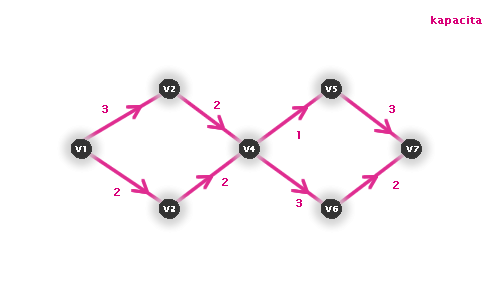
\includegraphics[width=0.7\textwidth]{img/net1.png}
  \end{figure}
  
  \item Najděte maximální tok z $v_1$ do $v_6$.
  \begin{figure}[!htbp]
    \centering
    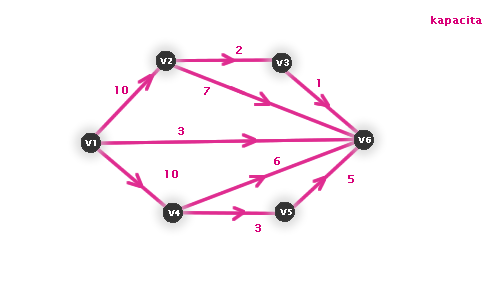
\includegraphics[width=0.7\textwidth]{img/net2.png}
  \end{figure}
  
  \item Najděte maximální tok z $v_1$ do $v_6$.
  \begin{figure}[!htbp]
    \centering
    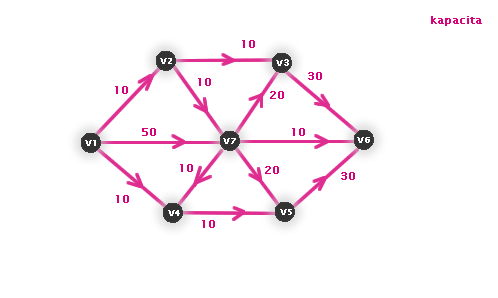
\includegraphics[width=0.7\textwidth]{img/net3.png}
  \end{figure}
  
  \item Najděte maximální tok z $v_1$ do $v_5$.
  \begin{figure}[!htbp]
    \centering
    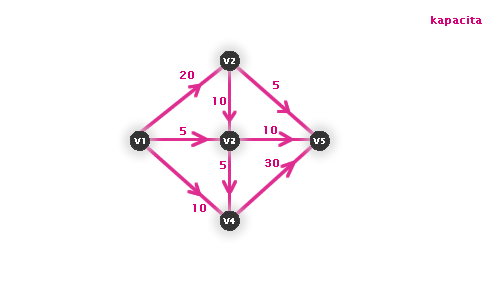
\includegraphics[width=0.7\textwidth]{img/net4.png}
  \end{figure}
  
  \item Najděte maximální tok z $v_1$ do $v_8$.
  \begin{figure}[!htbp]
    \centering
    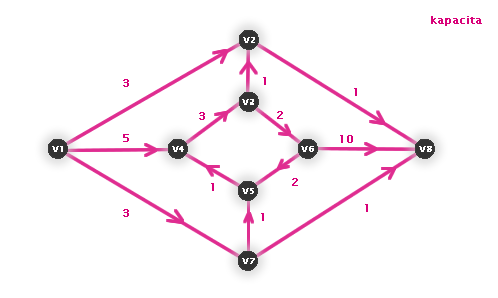
\includegraphics[width=0.7\textwidth]{img/net5.png}
  \end{figure}
\end{t_exercise}       % petrmanek
\section{Párování v bipartitních grafech}
\begin{t_example}
  Na začátek uvedeme motivační příklad. Jsme rozvrháři a snažíme se naplánovat přednášky na příští semestr. Máme konečnou množinu učitelů $U_1, U_2,\dots U_k$ a stejně velkou množinu předmětů $P_1, P_2,\dots P_k$. Jak už to ale bývá, ne každý učitel může (nebo chce) přednášet každý předmět, a tak nám každý učitel navíc dodá seznam přednášek, které mu můžeme přidělit.
  
  Celou situaci si můžeme hezky znázornit na bipartitním grafu, kde vrcholy jedné partity budou učitelé a v druhé budou předměty. Hranami spojíme každého učitele s předměty, které může vyučovat v příštím semestru. Z grafu chceme vybrat takový podgraf, že každý učitel je spojen s právě jedním předmětem.
\end{t_example}

\begin{t_definition}
  Párování v bipartitním grafu $G=(A\cup B,E)$ je množina hran $X\subseteq E$ taková, že žádné dvě hrany v ní nemají společný vrchol. Párování je perfektní, pokud hrany v $X$ sousedí se všemi vrcholy $G$. Velikostí párování míníme počet hran v $X$.
\end{t_definition}

Perfektní párování můžeme hledat pomocí teorie toků. Provedeme to tak, že z bipartitního grafu zkontstruujeme síť, v ní najdeme maximální tok a ten převedeme na párování. Síť zkonstruujeme takto:
\begin{enumerate}
  \item Vrcholy jedné partity připojíme ke zdroji, vrcholy druhé partity připojíme ke stoku.
  \item Zorientujeme hrany, aby šipky vedly od zdroje do připojené partity, z druhé připojené partity do stoku a ze zdojové partity do stokové partity.
  \item Každé hraně přidělíme stejnou kapacitu velikosti 1.
\end{enumerate}
Nyní už stačí jen najít maximální tok (třeba s pomocí Fordova-Fulkersonova algoritmu) a vytvořit z něj párování. Dříve jsme dokázali, že jsou-li kapacity celočíselné, i maximální tok bude celočíselný. Protože jsou navíc kapacity velikosti 1, může mít každá hrana tok jen 0 nebo 1 – do našeho párování tedy zahrneme pouze ty hrany s tokem 1.

Je triviální, že takto získané párování bude nejvýše maximální možné. Opačnou nerovnost získáme sporem. Pokud by nalezené párování bylo menší než maximální, musí existovat dvojice vrcholů, která šla spárovat. To také znamená, že mezi těmito vrcholy je nenulová rezerva, což je spor s maximalitou nalezeného toku. V důsledku tedy platí, že tímto způsobem nalezneme vždy maximální možné párování.

\begin{t_definition}
  Síť vytvořenou z bipartitního grafu $G$ budeme označovat jako síť přidruženou ke grafu $G$.
\end{t_definition}

\begin{t_claim}
  Pokud je bipartitní graf $G$ $k$-regulární, kde $k\geq 1$, potom v něm existuje perfektní párování.
\end{t_claim}

\begin{t_proof}
  Pozorujeme, že pokud je $G$ bipartitní a zároveň $k$-regulární, musí mít obě partity stejný počet vrcholů $n$. Chceme dokázat, že velikost maximálního toku v síti přidružené ke $G$ je rovna $n$.
  
  Vytvoříme tedy tok $f$ takový, že všechny hrany ze zdroje do partity nebo z partity do stoku budou mít tok 1 a všechny hrany mezi partitami budou mít tok $\frac{1}{n}$. Platí $|f|=n$, tento tok je tedy maximální možný (minimální řez je triviální). Jestliže existuje maximální tok velikosti $n$ na síti s celočíselnými kapacitami, existuje tok o stejné velikosti, který je celočíselný – z něj zkonstruujeme perfektní párování.
\end{t_proof}

Ukázali jsme si, jak najít perfektní párování. Co ale budeme dělat v případech, kdy takové párování neexistuje? Důkaz neexistence povedeme podle následujícího schématu.
\begin{enumerate}
  \item Vybereme podmnožinu $K$ vrcholů z partity $A$.
  \item Najdeme množinu $N(K)$ vrcholů spojených s vrcholy v $K$.
  \item Ukážeme, že $|K|\neq |N(K)|$, z čehož plyne, že perfektní párování nemůže existovat.
\end{enumerate}

\begin{t_definition}
  Vrcholové pokrytí grafu $G=(V,E)$ je taková množina $W\subseteq V$, že každá hrana v $E$ je incidentní s alespoň jedním vrcholem z $W$.
\end{t_definition}

\begin{t_remark}
  Triviální vrcholové pokrytí je množina všech vrcholů grafu. Často nás zajímá takzvané minimální vrcholové pokrytí, tedy vrcholové pokrytí s nejmenším možným počtem bodů. V bipartitním grafu o partitách velikosti $m$ a $n$ má minimální pokrytí velikost nejvýše $\min\{m,n\}$.
\end{t_remark}

\begin{t_theorem}[Königova]
  V každém bipartitním grafu je velikost maximálního párování rovna velikosti velikosti minimálního vrcholového pokrytí.
\end{t_theorem}

\begin{t_proof}
  Pokud je $W$ vrcholové pokrytí, musí hrany vedoucí mezi vrcholy této množiny, zdrojem a stokem tvořit stejně velký řez, protože každá $st$-cesta obsahuje alespoň jednu hranu bipartitního grafu a ta je pokryta. Analogicky, vezmeme-li libovolný $st$-řez (ne nutně tokový, stačí hranový), můžeme ho bez zvětšení upravit na $st$-řez, kterému přímočaře odpovídá vrcholové pokrytí stejné velikosti.
\end{t_proof}

Pojďme nyní prozkoumat souvislost párování a množinových systémů.

\begin{t_definition}
  Nechť $(X,\mathcal{L})$ je množinový systém, kde $\mathcal{L}=\{L_1,L_2,\dots L_k\}$. Množina $\{x_1,x_2,\dots x_k\}$ je systémem různých reprezentantů $(X,\mathcal{L})$, pokud pro každé $1\leq i\leq k$ platí $x_i\in L_i$.
\end{t_definition}

\begin{t_remark}
  Problém hledání systému různých reprezentantů v množinovém systému můžeme převést na hledání párování velikosti $|\mathcal{L}|$ na incidenčním grafu množinového systému. Tuto myšlenku rozvedeme v důkazu následující věty.
\end{t_remark}

\begin{t_theorem}[Hallova]
  Množinový systém $(X,\mathcal{L})$, kde $\mathcal{L}=\{L_1,L_2,\dots,L_k\}$, má systém různých reprezentantů, právě když pro každou $M\in 2^\mathcal{L}$ platí:
  \begin{align*}
    \left|\bigcup_{L_i\in M} L_i\right|\geq |M|
  \end{align*}
\end{t_theorem}

\begin{t_proof}
  Začneme jednodušší implikací, nechť v $(X,\mathcal{L})$ existuje systém různých reprezentantů $\{x_1,x_2,\dots x_k\}$. Chceme ukázat, že platí Hallova podmínka. Zvolíme libovolnou $M\in2^\mathcal{L}$. Pro každý prvek $L_i\in M$ existuje $x_i\in L_i$ takové, že všechna $x_i$ jsou navzájem různá. Proto:
  \begin{align*}
    \left|\bigcup_{L_i\in M} L_i\right|\geq |M|
  \end{align*}
  
  Nyní dokažme implikaci obrácenou. Mějme množinový systém $(X,\mathcal{L})$, který splňuje Hallovu podmínku. Vezmeme incidenční graf množinového systému a prozkoumáme jeho přidruženou síť. Nechť bez újmy na obecnosti je v této síti zdrojovou partitou množina $\mathcal{L}$ a stokovou partitou množina $X$. V síti nalezneme maximální tok $f$ a minimální řez $C^\prime$.
  
  ... \textit{(ukázat z řezu a Hallovy podmínky, že} $|f|=|\mathcal{L}|$) ... % todo
  
  Víme, že tok $f$ je celočíselný a má velikost $|\mathcal{L}|$. V incidenčním grafu tedy musí existovat párování velikosti $|\mathcal{L}|$. Systém různých reprezentantů získáme tak, že každé množině z $\mathcal{L}$ přiřadíme prvek z $X$, do kterého vede hrana s nenulovým tokem.
\end{t_proof}

\begin{t_corollary}
  Buď $G=(A\cup B,E)$ bipartitní graf s neprázdnou množinou hran $E$ takový, že pro libovolné dva vrcholy $a\in A$ a $b\in B$ platí $\deg_G a\geq \deg_G b$. Potom existuje párování, které má velikost $|A|$. 
\end{t_corollary}

\begin{t_proof}
  Definujeme množinový systém $\mathcal{M}=(B,\{N(a)\mid a\in A\})$. Řečeno slovy, pro každý vrchol z partity $A$ vytvoříme množinu vrcholů z partity $B$, které s ním sousedí. Nyní ukážeme, že v $\mathcal{M}$ platí Hallova podmínka.
  
  Zvolme libovolnou množinu $X\in 2^A$ vrcholů z první partity, označme $N(X)=\bigcup_{x\in X}N(x)$ množinu všech vrcholů z $B$ sousedících s vrcholy v $X$. Hallova podmínka vyžaduje, aby platilo $|N(X)|\geq |X|$, což nyní ověříme. Označme proměnné $k_1=\min_{x\in X}\{\deg_G x\}$ a $k_2=\max_{x\in N(X)}\{\deg_G x\}$. Počet hran mezi $X$ a $N(X)$ je přinejmenším $k_1|X|$ a také nejvýše $k_2|N(X)|$, platí tedy $k_1|X|\leq k_2|N(X)|$. Protože $k_1$ a $k_2$ jsou stupně vrcholů, platí podle předpokladu věty $k_1\geq k_2$ a dostáváme $|X|\leq |N(X)|$.
  
  Množinový systém $\mathcal{M}$ tedy má podle Hallovy věty systém různých reprezentantů. Tedy pro každý vrchol $a\in A$ existuje $b\in B$ tak, že mezi nimi povede hrana a všechna $b$ budou navzájem různá. To je přesně definice párování, které má velikost $|A|$.
\end{t_proof}

\begin{t_remark}
  Pokud hrany párování $X$ jsou sousedí se všemi vrcholy množiny $M$, také říkáme, že $X$ uspokojuje $M$.
\end{t_remark}

\begin{t_definition}
  Latinský čtverec $A$ je čtvercová matice typu $n\times n$ taková, že platí:
  \begin{enumerate}
    \item $a_{ij}\in\{1,2\dots n\}$,
    \item $a_{ij}\neq a_{i^\prime j}$ pro každé $i\neq i^\prime$,
    \item $a_{ij}\neq a_{ij^\prime}$ pro každé $j\neq j^\prime$.
  \end{enumerate}
\end{t_definition}

\begin{t_remark}
  Česky řečeno, v latinském čtverci se vyskytují přirozená čísla od jedné do $n$ taková, že v každém řádku i sloupci nenajdeme dvě stejná čísla.
\end{t_remark}

\begin{t_definition}
  Latinský obdélník $A$ je matice typu $k \times n$ splňující stejné podmínky jako latinský čtverec.
\end{t_definition}

\begin{t_claim}
  Každý latinský obdélník, kde je počet řádků $k$ nižší než počet sloupců $n$, lze doplnit na latinský čtverec.
\end{t_claim}

\begin{t_proof}
  K latinskému obdélníku budeme postupně přidávat řádky, dokud nedostaneme čtverec. Sestrojíme bipartitní graf $G=(S\cup H, E)$, kde $S=\{S_1, S_2, \dots S_n\}$ je množina sloupců latinského obdélníku ($\forall i:|S_i|=k$) a $H=\{1,2\dots n\}$ je množina hodnot, ze kterých konstruujeme nový řádek. Hrana v $G$ povede mezi $S_i\in S$ a $h\in H$, pokud se hodnota $h$ nevyskytuje ve sloupci $S_i$.
  
  Nyní chceme do nového řádku na $j$-tou pozici vybrat takovou hodnotu $h$, že se $h$ jednak nevyskytuje v sloupci $S_j$ a jednak všechny takto vybrané prvky $h$ jsou navzájem různé. To je však ekvivalentní s existencí systému různých reprezentantů na množinovém systému s incidenčním grafem $G$. Místo ověřování Hallovy podmínky se nám však tentokrát bude hodit využít předchozí tvrzení.
  
  Uvažme vrcholy v partitě $S$. V každém sloupci zadaného obdélníka chybí právě $n-k$ hodnot, platí tedy $\forall i:\deg_G S_i=n-k$. Naopak, každá hodnota chybí právě v $n-k$ sloupcích, platí tedy $\forall h\in H:\deg_G h=n-k$. Protože $n-k\leq n-k$, je podle předchozího tvrzení Hallova podmínka splněna a existuje párování v $G$ a tedy i hledaný systém různých reprezentantů.
\end{t_proof}

\begin{t_definition}
  Dva latinské čtverce $A$ a $B$ řádu $n$ označíme jako ortogonální, pokud platí
  $|\{(a_{ij},b_{ij})\mid 1\leq i,j \leq n\}|=n^2$.
\end{t_definition}

\begin{t_remark}
  Předchozí definici si můžeme lépe představit tak, že vezmeme čtverce $A$, $B$ a překryjeme je přes sebe tak, že nám prvky na odpovídajících pozicích vytvoří uspořádané dvojice. Protože se v těchto dvojicích mohou na obou místech vyskytovat čísla od jedné do $n$, může jich být až $n^2$. Definice tedy vlastně říká, že se mezi těmito uspořádanými dvojicemi nesmí žádná opakovat vícekrát.
\end{t_remark}

\begin{t_theorem}
  Nechť je $M$ množinou latinských čtverců řádu $n$, z nichž každé dva jsou nazvájem ortogonální. Potom $|M|\leq n-1$.
\end{t_theorem}

\begin{t_proof}
  Začneme pozorováním. Mějme $A, B$ ortogonální latinské čtverce řádu $n$ a $\pi$ permutaci čísel $\{1, 2,\dots n\}$. Utvoříme nový latinský čtverec $A^\prime$ tak, že $a^\prime_{ij}=\pi(a_{ij})$. Z definice ortogonality není těžké nahlédnout, že potom i $A^\prime$ a $B$ budou ortogonální latinské čtverce.
  
  Nechť $A_1,A_2,\dots A_t$ jsou latinské čtverce řádu $n$, z nichž každé dva jsou ortogonální. Pro každé $A_i$ zvolíme tu permutaci čísel $\{1,2,\dots n\}$, jejíž aplikací na $A_i$ docílíme toho, že v první řádce budou stát čísla $1,2,\dots n$ v pořadí podle velikosti. Výsledný čtverec označíme $A^\prime_i$. Podle uvedeného pozorování budou $A^\prime_1,\dots A^\prime_t$ stále po dvou ortogonální. Podívejme se nyní, jaká čísla mohou stát v prvním políčku druhé řádky těchto čtverců. Především tam nemůže být číslo 1, protože to už je v prvním sloupci použito. Dále, žádné dva čtverce $A^\prime_i, A^\prime_j$ nemůžou mít na uvažované pozici stejná čísla. Kdyby totiž měly, položením čtverců přes sebe vznikne dvojice stejných čísel, řekněme $(k,k)$, ale tato dvojice také vznikne na $k$-tém místě prvního řádku! Tedy každé z čísel $2,3,\dots n$ může na pozici $a_{21}$ stát jen v jednom $A^\prime_i$, a proto $t\leq n-1$.
\end{t_proof}

\begin{t_theorem}
  Pro $n\geq 2$, konečná projektivní rovina řádu $n$ existuje právě když existuje soubor $n-1$ po dvou ortogonálních latinských čtverců řádu $n$.
\end{t_theorem}

\begin{t_proof}[Myšlenka důkazu]
  Máme dáno $n-1$ ortogonálních latinských čtverců $L_1,L_2\dots L_{n-1}$ řádu $n$. Zvolíme dva body projektivní roviny $r$ a $s$, přímku $B$, která je spojuje, a zbývající body na přímce $B$ označíme $l_1,\dots l_{n-1}$. Potom nazveme $R_1\dots R_n$ zbývající přímky procházející bodem $r$, a $S_1,\dots S_n$ zbývající přímky procházející bodem $s$ (mimo $B$).
  
  Nyní každý z dosud neoznačených bodů je průsečíkem některé dvojice přímek $R_i$ a $S_j$. Body konstruované projektivní roviny mimo bodů $r, s, l_1,\dots l_{n-1}$ máme sestaveny do čtverce $n\times n$; pozice bodu v tomto čtverci bude odpovídat pozici políčka v latinském čtverci. Například pole $a_{32}$ bude odpovídat průsečíku $R_3$ a $S_2$.
  
  To, co jsme dosud označili a zakreslili, musí být stejné v každé projektivní rovině řádu $n$. Nyní podle latinských čtverců doplníme přímky procházející body $l_1\dots l_{n-1}$. Jak označení napovídá, přímky procházející bodem $l_i$ budou určeny čtvercem $L_i$. Přímky bodem $l_i$ budou odpovídat jednotlivým číslům (symbolům) v latinském čtverci $L_i$. Například přímka odpovídající číslu 1 bude protínat bod $l_1$ a všechny průsečíky $R_i$ a $S_j$ odpovídající polím $a_{ij}$ ve čtverci $L_1$ takovým, že $a_{ij}=1$. Pro ostatní čísla postupujeme analogicky.
  
  Tím jsme popsali konstrukci konečné projektivní roviny, zbývá ověřit axiomy. Snadno spočteme, že celkový počet bodů i přímek je $n^2+n+1$. Stačí ověřit, že každé 2 přímky se protínají nejvýš v 1 bodě. Přitom se využije toho, že každý $L_i$ je latinský čtverec a každé 2 z použitých čtverců jsou ortogonální.
  
  Obrácený postup, konstrukce $n-1$ po dvou ortogonálních latinských čtverců z projektivní roviny, sleduje totéž schéma. V projektivní rovině libovolně zvolíme body $r, s$ a zafixujeme další označení. Potom $i$-tý latinský čtverec vyplníme podle přímek procházejících bodem $l_i$.
\end{t_proof}

\begin{t_exercise}
  \item Uvažujme systém všech $(n-1)$-prvkových podmnožin množiny $\{1, 2\dots n\}$. Kolik má systémů různých reprezentantů?
  \item Dokažte, že systém všech podmnožin velikosti $(n-2)$ množiny $\{1,2\dots n\}$ má systém různých reprezentantů.
  \item Určete, zda pro množinový systém $(X,\mathcal{L})$ existuje systém různých reprezentantů:\\
  $X=\{a,b,c,d\}$, $\mathcal{L}=\{\{a,b,d\}, \{a,c\}, \{b,c\}, \{b,d\}\}$
  \item Určete, zda pro množinový systém $(X,\mathcal{L})$ existuje systém různých reprezentantů:\\
  $X=\{a,b,c\}$, $\mathcal{L}=\{\{a,c\}, \{a,c\}, \{b,c\}, \{a,b\}\}$
  \item Určete, zda pro množinový systém $(X,\mathcal{L})$ existuje systém různých reprezentantů:\\
  $X=\{a,b,c,d,e,f\}$, $\mathcal{L}=\{\{a,b\}, \{a,e\}, \{b,c\}, \{a,b,d\}, \{a,c\}, \{b,e,f\}, \{a,b,c\}\}$
  \item Dokažte, že množinový systém sestávající z přímek konečné projektivní roviny má vždy systém různých reprezentantů.
  \item Existují 3 navzájem ortogonální latinské čtverce řádu 5? Pokud si myslíte že ano, zkuste je sestrojit, pokud ne, zdůvodněte proč.
  \item Doplňte následující tabulku na latinský čtverec nebo dokažte, že to nejde.
  \begin{table}[h]
    \centering
    \begin{tabular}{|l|l|l|l|l|l|}
      \hline
      1 & 2 & 3 & 4 & 5 & 6 \\ \hline
        &   &   &   &   &   \\ \hline
      6 & 3 & 5 & 1 & 2 & 4 \\ \hline
        &   &   &   &   &   \\ \hline
        &   &   &   &   &   \\ \hline
      2 & 1 & 6 & 5 & 4 & 3 \\ \hline
    \end{tabular}
  \end{table}
\end{t_exercise}   % petrmanek
\section{Grafová souvislost}
\begin{t_definition}
  V grafu $G=(V,E)$ je množina $F\subseteq E$ $st$-řezem (kde $s,t\in V$), pokud jsou v grafu $G-F$ vrcholy $s$ a $t$ v různých komponentách souvislosti. Obecně, množina $F^\prime\subseteq E$ je řezem, pokud existují $s,t\in V$ takové, že $F^\prime$ je $st$-řezem.
\end{t_definition}

\begin{t_definition}
  V grafu $G=(V,E)$ je množina $W\subseteq V$ $st$-separátorem (kde $s,t\in V$ a $s,t\notin W$), pokud jsou v grafu $G-W$ vrcholy $s$ a $t$ v různých komponentách souvislosti. Obecně, množina $W^\prime\subseteq E$ je separátorem, pokud existují $s,t\in V$ takové, že $W^\prime$ je $st$-separátorem.
\end{t_definition}

\begin{t_definition}
  Graf $G$ nazýváme $k$-hranově souvislý, pokud v něm neexistuje řez velikosti $k-1$ nebo menší. Podobně, $G$ označíme jako $k$-vrcholově souvislý, pokud v něm neexistuje separátor velikosti $k-1$ nebo menší a $G$ má alespoň $k+1$ vrcholů.
\end{t_definition}

\begin{t_remark}
  Každý $k$-souvislý graf je i $(k-1)$-souvislý (hranově i vrcholově).
\end{t_remark}

\begin{t_definition}
  Hranová souvislost grafu $G$, označena $k_e(G)$, je největší $k$ takové, že $G$ je $k$-hranově souvislý. Podobně, vrcholová souvislost $k_v(G)$ je největší $l$ takové, že $G$ je $l$-vrcholově souvislý.
\end{t_definition}

\begin{t_observation}
  V každém grafu $G$ existuje řez velikosti $k_e(G)$ a separátor velikosti $k_v(G)$. Z definice vyplývá, že tyto množiny jsou minimálními možnými.
\end{t_observation}

\begin{t_theorem}[Mengerova, lokální hranová orientovaná]
  Buď $G=(V,E)$ orientovaný graf a $s, t\in V$ nějaké jeho vrcholy. Pak je velikost minimálního $st$-řezu rovna počtu navzájem hranově disjunktních cest z $s$ do $t$.
\end{t_theorem}

\begin{t_proof}
  Z grafu sestrojíme síť takovou, že $s$ bude zdroj, $t$ bude stok a všem hranám nastavíme kapacitu na jednotku. Řezy v této síti odpovídají řezům v původním grafu. Nyní aplikujeme Fordovu-Fulkersonovu větu na minimální $st$-řez a získáme maximální tok $f$ o stejné velikosti.
  
  Pozorujeme, že každý systém hranově disjunktních cest z $s$ do $t$ odpovídá toku stejné velikosti a naopak ke každému celočíselnému toku dovedeme najít systém disjunktních cest (hladově tok rozkládáme na cesty a průběžně odstraňujeme hrany s nulovým tokem, které objevíme). Tento proces aplikujeme na $f$ a získáme hledané cesty.
\end{t_proof}

\begin{t_theorem}[Mengerova, lokální vrcholová orientovaná]
  Buď $G=(V,E)$ orientovaný graf a $s, t\in V$ nějaké jeho vrcholy takové, že $(s,t)\notin E$. Pak je velikost minimálního $st$-separátoru rovna maximálnímu počtu cest z $s$ do $t$, které jsou vrcholově disjunktní až na krajní body.
\end{t_theorem}

\begin{t_proof}
  Podobně jako v předchozím důkazu zkonstruujeme vhodnou síť. Tentokrát ovšem rozdělíme každý vrchol $v\in V$ na vrcholy $v^+$ a $v^-$. Všechny hrany, které původně vedly do $v$ přepojíme do $v^+$ a hrany vedoucí z $v$ povedou z $v^-$. Navíc přidáme novou hranu z $v^+$ do $v^-$. Všechny hrany budou mít jednotkové kapacity.
  
  Toky v takto utvořené síti nyní odpovídají vrcholově disjunktním cestám, řezy v síti odpovídají $st$-separátorům. Analogicky k minulému důkazu najdeme k minimálnímu separátoru maximální tok, ten převedeme na hledané cesty a důkaz je hotov.
\end{t_proof}

\begin{t_corollary}[Mengerova věta, globální hranová neorientovaná]
  Neorientovaný graf $G$ je hranově $k$-souvislý právě tehdy, když mezi každými dvěma vrcholy existuje alespoň $k$ hranově disjunktních cest.
\end{t_corollary}

\begin{t_corollary}[Mengerova věta, globální vrcholová neorientovaná]
  Neorientovaný graf $G$ je vrcholově $k$-souvislý právě tehdy, když mezi každými dvěma vrcholy existuje alespoň $k$ vrcholově disjunktních cest až na krajní body.
\end{t_corollary}

\begin{t_definition}
  V grafu $G=(V,E)$ označíme:
  \begin{itemize}
    \item \textit{Minimální stupeň} $\delta(G)=\min_{v\in V}\{\deg_G v\}$,
    \item \textit{Maximální stupeň} $\Delta(G)=\max_{v\in V}\{\deg_G v\}$.
  \end{itemize}
\end{t_definition}

\begin{t_theorem}
  V každém grafu $G=(V,E)$, kde $e\in E$, platí: $k_v(G)-1\leq k_v(G-e)\leq k_v(G)$.
\end{t_theorem}

\begin{t_proof}
  chybí % todo
\end{t_proof}

\begin{t_corollary}
  V každém grafu $G=(V,E)$ platí: $k_v(G)\leq k_e(G)\leq \delta(G)$.
\end{t_corollary}

\begin{t_lemma}
  Nechť $G=(V,E)$ je graf, potom platí:
  \begin{align*}
    \frac{\Delta(G)}{2}\cdot k_v(G) \geq k_e(G)
  \end{align*}
\end{t_lemma}

\begin{t_proof}
  chybí % todo
\end{t_proof}

\begin{t_definition}
  Nechť $G=(V,E)$ je graf. Cesta $P\subseteq G$ je ucho, pokud její vnitřní vrcholy nesousedí s žádným jiným vrcholem v $G$.
\end{t_definition}

\begin{t_lemma}[ušaté]
  Každý 2-vrcholově souvislý graf může být vytvořen z cyklu postupným přidáváním uší.
\end{t_lemma}

\begin{t_proof}
  Protože $G=(V,E)$ je 2-vrcholově souvislý, platí $\delta(G)\geq 2$ a tedy v $G$ musí existovat cyklus, označme jej $C$. Indukcí ukážeme pro $n\leq|E|$, že existuje podgraf $H\subseteq G$ na alespoň $n$ hranách takový, že jej můžeme vytvořit postupným přidáváním uší k $C$.
  \begin{enumerate}
    \item[(0)] Pro $n=0$ je hledaným grafem $C$.
    \item[(1)] Podle indukčního předpokladu existuje podgraf $H=(V^\prime,E^\prime)\subseteq G$ na alespoň $n-1$ hranách s požadovanou vlastností. Pokud $|E^\prime|\geq n$, jsme hotovi. Předpokládejme tedy, že $H$ má právě $n-1$ hran.
    
    Pokud existuje hrana $e=(x,y)\in E\setminus E^\prime$ taková, že $x,y\in V^\prime$, vytvoříme graf $H+e$ na $n$ hranách. Protože jednotlivá hrana splňuje definici ucha, je $H+e$ grafem s požadovanou vlastností.
    
    Pokud taková hrana neexistuje, je $H$ indukovaným podgrafem $G$, takže množina $X=\{(x,y)\mid x\in V^\prime, y\in V\setminus V^\prime\}$ tvoří řez v $G$ (protože $|V^\prime|\geq n$). Zvolíme libovolnou hranu $e\in X$. Protože $G$ je 2-vrcholově souvislý, musí podle Mengerovy věty v $G$ existovat další cesta $P$ mezi krajními vrcholy $e$. Spojíme hranu s cestou a vytvoříme množinu $W=P+e$. Nahlédneme, že $W$ je ucho délky alespoň 1. Graf $H+W$ tedy splňuje požadovanou vlastnost.
  \end{enumerate}
\end{t_proof}

\begin{t_definition}
  Počet koster grafu $G$ označíme $\kappa(G)$.
\end{t_definition}

\begin{t_theorem}
  Pokud je graf $G=(V,E)$ 2-vrcholově souvislý, potom $\kappa(G)\geq |V|$.
\end{t_theorem}

\begin{t_proof}
  chybí % todo
\end{t_proof}

\begin{t_theorem}[Cayleyova formule]
  Pro úplný graf $K_n$ na $n$ vrcholech platí: $\kappa(K_n)=n^{n-2}$.
\end{t_theorem}

\begin{t_proof}
  Uvažme množinu všech posloupností čísel $\{1,2,\dots n\}$ délky $n-2$. Je jednoduché nahlédnout, že takových posloupností je $n^{n-2}$. Nyní najdeme bijekci mezi těmito posloupnostmi a kostrami grafu $K_n$.
  
  Pro převedení kostry $T\subseteq K_n$ na posloupnost použijeme následující algoritmus:
  \begin{enumerate}
    \item Z množiny vrcholů stupně 1 vybereme vrchol $v$ s nejnižším číslem. Vrchol $v$ odebereme z $T$ a zapíšeme do posloupnosti číslo jeho jediného souseda.
    \item Získali jsme nový, o jeden vrchol menší graf. Na něm budeme stejný postup opakovat, dokud nám nezbyde graf na jednom vrcholu.
  \end{enumerate}
  
  Tímto způsobem získáme posloupnost délky $n-1$. Víme, že poslední prvek bude vždy číslo $n$, protože i kdyby na začátku $\deg_T n=1$, ve stromě bude vždy ještě alespoň jeden další vrchol stupně 1 s nižším číslem. Z tohoto důvodu můžeme poslední prvek posloupnosti vynechat a zkrátit ji tak na délku $n-2$, což je přesně posloupnost, do které jsme chtěli kostru převést.
  
  Pojďme nyní ukázat, že zobrazení, které výše uvedeným způsobem přiřadí kostře posloupnost, je opravdu bijekcí. Pozorujeme, že žádný z vrcholů stupně 1 se v posloupnosti neobjeví. Obecněji, každý vrchol $v$ se v posloupnosti vyskytne právě $(\deg_T v-1)$-krát. To nám dává návod, jak z posloupnosti zrekonstruujeme původní graf $T$.
  \begin{enumerate}
    \item Najdeme vrchol s nejnižším číslem, které se v posloupnosti nevyskytuje, a připojíme ho hranou k vrcholu určenému prvním číslem v posloupnosti.
    \item Odebereme první číslo z posloupnosti, čímž získáme menší posloupnost. Na ní budeme opakovat stejný postup, dokud nevyčerpáme celou posloupnost.
    \item Vrchol určený posledním číslem v posloupnosti připojíme k vrcholu $n$.
  \end{enumerate}
  
  Je vidět, že každou posloupnost umíme převést zpět na graf a naše zobrazení je tedy určitě na. Protože jsme navíc při obou procesech měli každý krok určen jednoznačně (když bylo více vrcholů, volili jsme ten menší), je zobrazení prosté, čili máme bijekci.
\end{t_proof}

\begin{t_remark}
  Výše popsaná bijekce se nazývá Prüferova posloupnost.
\end{t_remark}

\begin{t_theorem}
  Pokud graf $G=(V,E)$ neobsahuje trojúhelník, potom $|E|\leq \frac{|V|^2}{4}$.
\end{t_theorem}

\begin{t_proof}
  chybí % todo
\end{t_proof}

\begin{t_theorem}
  Pokud graf $G=(V,E)$ neobsahuje 4-cyklus, potom $|E|\leq \frac{\sqrt{2}}{2}|V|^\frac{3}{2}$.
\end{t_theorem}

\begin{t_proof}
  chybí % todo
\end{t_proof} % petrmanek
\section{Ramseyova teorie}     % petrmanek
% todo:  kombagra/8kody -------- petrmanek

\section{Párování 2}
\begin{t_definition}
  Buď $G=(V,E)$ graf. Párování v $G$ je množina hran $M \subseteq E$ taková, že každý vrchol sousedí nejvýše s 1 hranou $M$. \\
\end{t_definition}
\begin{t_definition}
  Volný vrchol v párování $M$ je vrchol, který není v žádné párovací hraně, tedy $\forall e \in M: \; v \not\in e$.
\end{t_definition}
\begin{t_definition}
  Párování $M$ je největší (anglicky maximum), pokud neexistuje párování $M'$, kde $|M'| > |M|$.
\end{t_definition}
\begin{t_definition}
  Párování $M$ je maximální (anglicky maximal), pokud neexistuje párování $M'$, kde $M \neq M'$ a $M \subseteq M'$.
\end{t_definition}
\begin{t_definition}
  Párování $M$ je perfektní, pokud nemá žádný volný vrchol.
\end{t_definition}
\begin{t_definition}
  Mějme $G=(V,E)$ graf, $M$ párování v $G$. Střídavá cesta vzhledem k $M$ je cesta v $G$, na níž se střídají párovací a nepárovací hrany.
\end{t_definition}
\begin{t_definition}
  Volná střídavá cesta (VSC) (jinak také zlepšující cesta, neboli augmenting path) je střídavá cesta, která spojuje 2 volné vrcholy.
\end{t_definition}
\begin{t_lemma}
  Buď $G=(V,E)$ graf, $M$ jeho párování. Pak $M$ je největší $\iff$ $M$ nemá VSC.
\end{t_lemma}
\begin{t_proof}
  Implikaci zleva doprava ukážeme jednoduše sporem. Pokud by $M$ mělo VSC, vyměníme v té VSC párovací hrany za nepárovací a naopak. Tím jsme dostali párování, které má o jednu párovací hranu více, což je spor s tím, že $M$ bylo největší párování. \\
  Opačná implikace obměnou: Nechť M není největší. Volme tedy $M'$ párování v $G$ takové, že $|M'| > |M|$. Označme si $N = M \triangle M'$ a uvažme graf $H=(V,N)$. Pozorování: 
  \begin{itemize}
    \item V tomto grafu má každý vrchol stupeň nejvýše 2, což vyplývá z volby množiny hran, tedy každá komponenta $H$ je cesta anebo kružnice. 
    \item Každá kružnice má stejný počet hran z $M$ jako z $M'$. 
    \item Platí $|M'| > |M|$ \implies existuje komponenta $H$, která má více hran z $M'$ než z $M$. Tato komponenta je však VSC pro $M$.
  \end{itemize}
\end{t_proof}
  Již tedy víme něco o párování, chtěli bychom tedy algoritmus, který nalezne největší párování.
\begin{t_observation}
  Stačí algoritmus, který pro zadaný $G$ a jeho párování $M$ najde větší párování, nebo rozhodne, že takové neexistuje.
\end{t_observation}
\begin{t_definition}
  Kytka v grafu $G$ s párováním $M$ je podgraf, který je složen z kružnice $C_i$, která má lichou délku a právě $\lfloor i/2 \rfloor$ párovacích hran, a střídavé cesty sudé délky, která má na svém konci volný vrchol a její druhý konec je vrchol na kružnici $C_i$. Kružnici nazýváme \textit{květ} a cestu \textit{stonek}. Pozorujeme, že z květu vychází nejvýše jedna párovací hrana do stonku. (Kytka nemusí mít stonek.)
\end{t_definition}
\begin{t_definition}
  Kontrakce květu $K$ je operace, kde všechny vrcholy kružnice nahradíme jedním novým vrcholem $V_K$, jehož sousedé jsou sjednocení sousedů všech vrcholů květu $K$. Graf vzniklý kontrakcí květu značíme $G.K$ a jeho párování $M.K$
\end{t_definition}
\begin{t_lemma}
  \begin{enumerate}
    \item $G$ je graf, $K$ květ kytky v $M$. Pak $M$ je největší v $G$ $\iff$ $M.K$ je největší v $G.K$.
    \item Když najdeme v $G.K$ párování $M'$ větší, než $M.K$, tak z něj umíme získat v polynomiálním čase párování $M''$ v grafu $G$, které je větší, než $M$.
  \end{enumerate}
\end{t_lemma}
\begin{algorithm}
  \caption{Edmonsův kytičkový (blossom) algoritmus (1963)}
  Kostra algoritmu: \\
  Zkus najít VSC anebo kytku v $(G,M)$. 
    \begin{itemize}
      \item Pokud najdeš VSC, tak zlepši $M$.
      \item Pokud najdeš kytku, zavolej se na $(G.K, M.K)$ Pokud $M.K$ lze zlepšit, zlepši $M$, jinak konec.
    \end{itemize}
  \end{enumerate}
  Pokud už není ani VSC ani kytka, konec. \\
  \textbf{Algoritmus:} \\
  Vstup: graf $G$, párování $M$.
  \begin{enumerate}
    \item Vytvoř frontu vrcholů $F = \emptyset$, les $L = \emptyset$. 
    \item Najdi volné vrcholy, vlož je do $F$ a do $L$ na hladinu 0.
    \item Dokud $F \neq \emptyset$:
    \item Vyjmi první vrchol z fronty $F$, přiřaď ho do $v$ a označ $h$ hladinu $v$.
    \item Pokud je $h$ lichá, zvolím $y$ vrchol spojený s $v$ párovací hranou. Pokud $y \not\in L$, zařaď $y$ do $F$, přidej $y$ do $L$ spolu s $vy$ na hladinu $h+1$. Jinak $y \in L$, pak je $y$ na hladině $h$, tedy najdu VSC nebo $K$.
    \item Pokud je $h$ sudá, tak si zvolím $Y$ jako množinu vrcholů dosažitelných z $v$ po nepárovací hraně. Máme dvě možnosti - buď $\exists y \in Y, y \in L, h(y)$ je sudé $\implies$ najdu VSC, nebo $K$; anebo $\forall y \in Y$ nepatřící do $L$, zařaď $y$ do $F$, přidej $y$ a $vy$ do $L$ na hladinu $h+1$.
  \end{enumerate}
  Pokud se F se vyprázdní bez nalezení VSC nebo kytky, $M$ je největší párování.
\end{algorithm}
 % salmelu

\end{document}
